\section{Algorithms Benchmark}
\subsection{About Test Cases}
\begin{itemize}
    \item \textbf{Test cases description}
          \begin{itemize}
              \item Each map size in (7 × 7), (9 × 9), (11 × 11), (13 × 13), (17 × 17), (20 × 20) has at least 5 test cases with different difficulty levels. (There are also test cases for (3 × 3) and (5 × 5) for brute force algorithm.)
              \item The test cases are generated randomly and the difficulty levels are classified as easy, medium, hard, and very hard with the increasing of crossing edges, the number of islands with high degrees, etc. The results of the tests are shown in the table and figures below. The time is measured in milliseconds (ms) and the peak memory is measured in kilobytes (KB).
          \end{itemize}


    \item \textbf{Challenges}
          \begin{itemize}
              \item \textbf{Generating CNF}
                    \begin{itemize}
                        \item Generating CNF clauses for constraints like `degree constraints' is quite complex and time-consuming. The algorithm needs to consider all possible combinations of edges and nodes to generate the CNF clauses.
                    \end{itemize}
              \item \textbf{Algorithm implementations}
                    \begin{itemize}
                        \item The algorithm is not optimal for large maps, which leads to a long solving time and high peak memory usage.
                        \item The algorithm is not able to solve some test cases with a very high difficulty level.
                    \end{itemize}
          \end{itemize}
\end{itemize}

\subsection{Experiment results}
\begin{flushleft}
    \begin{itemize}
        \item \textbf{Brute Force}
              \begin{flushleft}
                  \begin{itemize}
                      \item The brute force algorithm is able to solve all test cases with a map size of (3 × 3) and (5 × 5) slowly. It is not able to solve larger maps due to the exponential growth of the search space.
                  \end{itemize}

                  \begin{table}[ht]
                      \centering
                      \begin{tabular}{|l|l|l|l|}
                          \hline
                          \textbf{Map Size} & \textbf{Time (s)} & \textbf{Memory}                                         \\
                          \hline
                          3 × 3             & 0.02              & \( 11704 \, \text{B} \) (\( \approx 11.38 \, \text{KB} \))   \\
                          \hline
                          5 × 5             & 413.68            & \( 75176 \, \text{B} \) (\( \approx 73.41 \, \text{KB} \))   \\
                          \hline
                          7 × 7             & 879.78            & \( 125816 \, \text{B} \) (\( \approx 122.86 \, \text{KB} \)) \\
                          \hline
                      \end{tabular}
                      \caption{Comparison of Time and Memory for Different Map Sizes}
                  \end{table}
              \end{flushleft}
        \item \textbf{Backtracking}
              \begin{itemize}
                  \item The backtracking algorithm is able to solve almost test cases with all map size in a reasonable time.
              \end{itemize}
        \item \textbf{A*}
              \begin{itemize}
                  \item The A* algorithm is able to solve all test cases with almost map size in a reasonable time. However, it is not able to solve some test cases with a very high difficulty level due to the large search space.
              \end{itemize}
        \item \textbf{PySAT}
              \begin{itemize}
                  \item The PySAT algorithm is able to solve all test cases with all map size in nearly instant time. It is the fastest algorithm among all algorithms.
              \end{itemize}
    \end{itemize}
\end{flushleft}

\pagebreak
\begin{figure}[!ht]
    \centering
    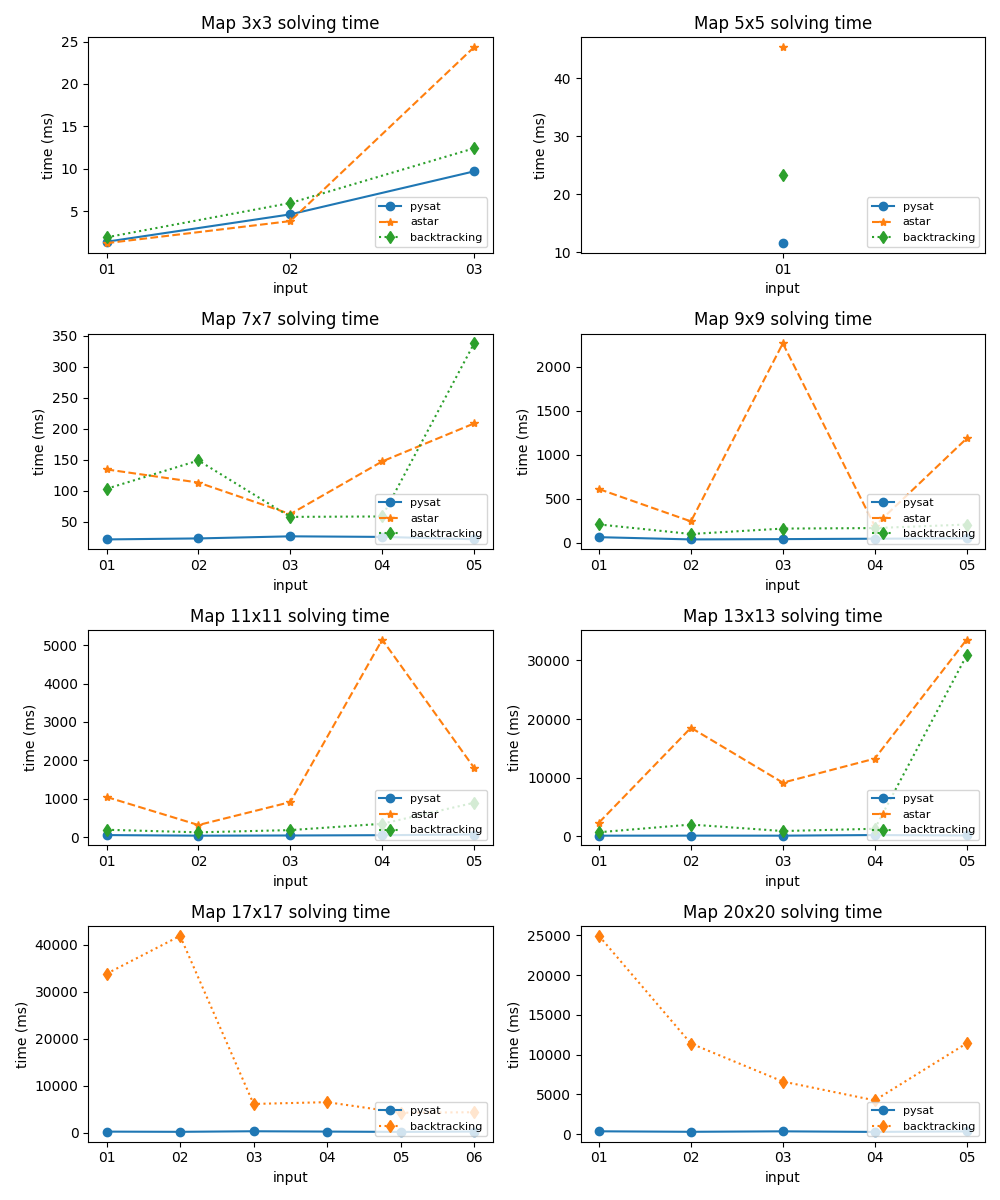
\includegraphics[width=0.95\textwidth]{imgs/benchmark-solving_time.png}
    \caption{Solving time Benchmark}
\end{figure}
\pagebreak
\begin{figure}[!ht]
    \centering
    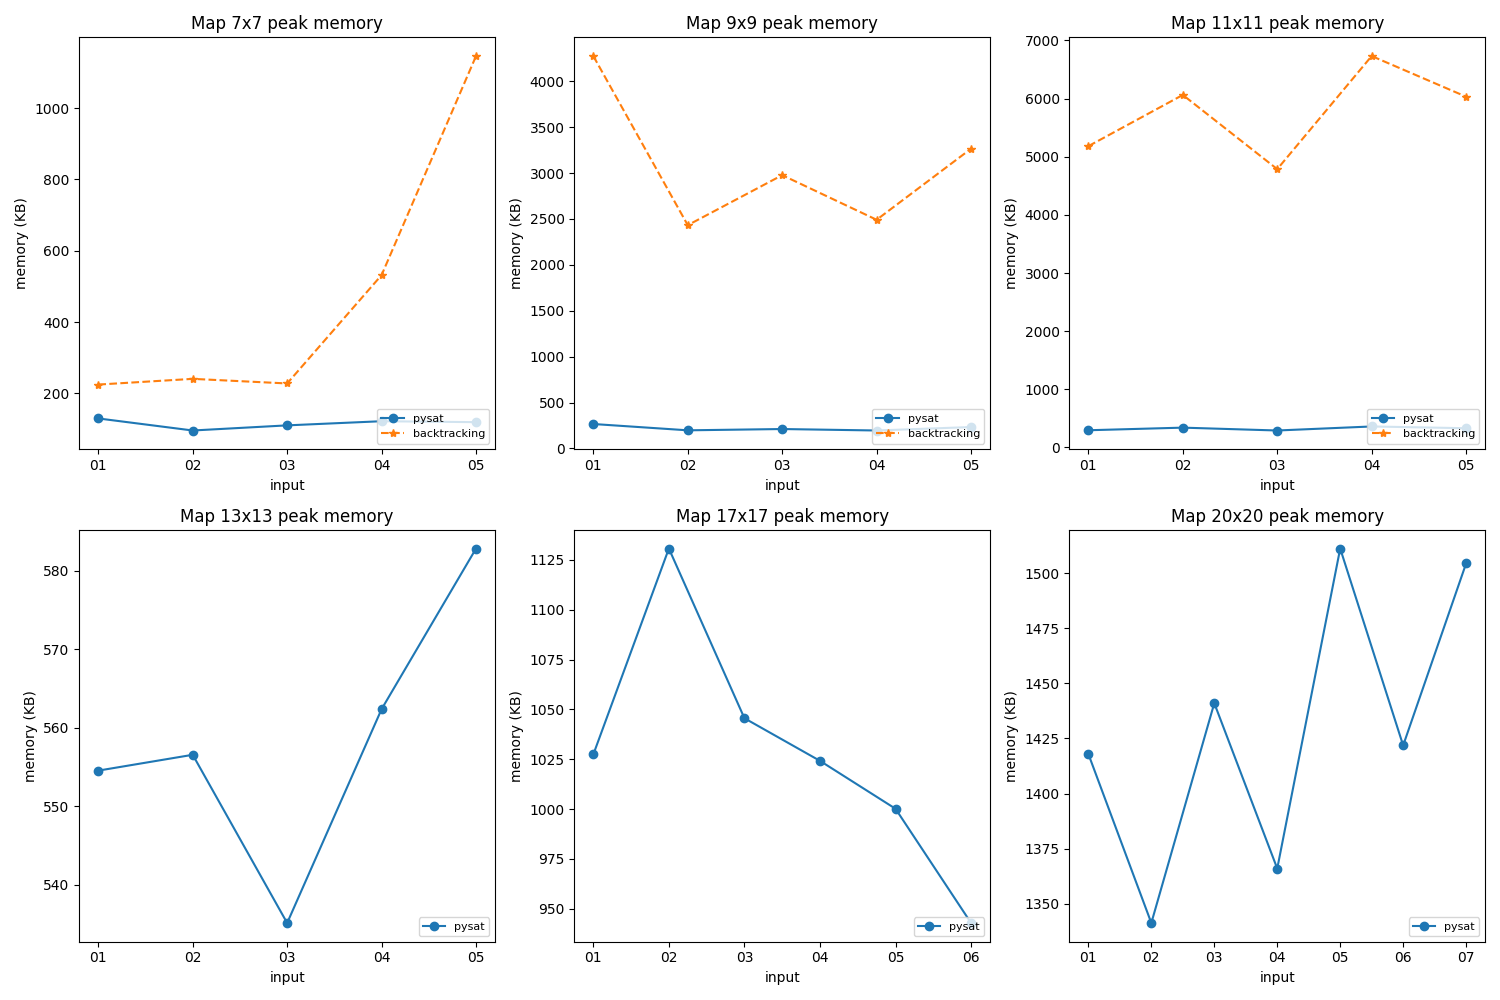
\includegraphics[width=0.95\textwidth]{imgs/benchmark-peak_memory.png}
    \caption{Solving time Benchmark}
\end{figure}
